\documentclass[
  shownotes,
  xcolor={svgnames},
  hyperref={colorlinks,citecolor=DarkBlue,linkcolor=DarkRed,urlcolor=DarkBlue}
  ]{beamer}
\usepackage{animate}
\usepackage{amsmath}
\usepackage{amsfonts}
\usepackage{amssymb}
\usepackage{pifont}
\usepackage{mathpazo}
%\usepackage{xcolor}
\usepackage{multimedia}
\usepackage{fancybox}
\usepackage[para]{threeparttable}
\usepackage{multirow}
\setcounter{MaxMatrixCols}{30}
\usepackage{subcaption}
\usepackage{graphicx}
\usepackage{lscape}
\usepackage[compatibility=false,font=small]{caption}
\usepackage{booktabs}
\usepackage{ragged2e}
\usepackage{chronosys}
\usepackage{appendixnumberbeamer}
\usepackage{animate}
\setbeamertemplate{caption}[numbered]
\usepackage{color}
%\usepackage{times}
\usepackage{tikz}
\usepackage{comment} %to comment
%% BibTeX settings
\usepackage{natbib}
\bibliographystyle{apalike}
\bibpunct{(}{)}{,}{a}{,}{,}
\setbeamertemplate{bibliography item}{[\theenumiv]}

% Defines columns for bespoke tables
\usepackage{array}
\newcolumntype{L}[1]{>{\raggedright\let\newline\\\arraybackslash\hspace{0pt}}m{#1}}
\newcolumntype{C}[1]{>{\centering\let\newline\\\arraybackslash\hspace{0pt}}m{#1}}
\newcolumntype{R}[1]{>{\raggedleft\let\newline\\\arraybackslash\hspace{0pt}}m{#1}}


\usepackage{xfrac}


\usepackage{multicol}
\setlength{\columnsep}{0.5cm}

% Theme and colors
\usetheme{Boadilla}

% I use steel blue and a custom color palette. This defines it.
\definecolor{andesred}{HTML}{af2433}

% Other options
\providecommand{\U}[1]{\protect\rule{.1in}{.1in}}
\usefonttheme{serif}
\setbeamertemplate{itemize items}[default]
\setbeamertemplate{enumerate items}[square]
\setbeamertemplate{section in toc}[circle]

\makeatletter

\definecolor{mybackground}{HTML}{82CAFA}
\definecolor{myforeground}{HTML}{0000A0}

\setbeamercolor{normal text}{fg=black,bg=white}
\setbeamercolor{alerted text}{fg=red}
\setbeamercolor{example text}{fg=black}

\setbeamercolor{background canvas}{fg=myforeground, bg=white}
\setbeamercolor{background}{fg=myforeground, bg=mybackground}

\setbeamercolor{palette primary}{fg=black, bg=gray!30!white}
\setbeamercolor{palette secondary}{fg=black, bg=gray!20!white}
\setbeamercolor{palette tertiary}{fg=white, bg=andesred}

\setbeamercolor{frametitle}{fg=andesred}
\setbeamercolor{title}{fg=andesred}
\setbeamercolor{block title}{fg=andesred}
\setbeamercolor{itemize item}{fg=andesred}
\setbeamercolor{itemize subitem}{fg=andesred}
\setbeamercolor{itemize subsubitem}{fg=andesred}
\setbeamercolor{enumerate item}{fg=andesred}
\setbeamercolor{item projected}{bg=gray!30!white,fg=andesred}
\setbeamercolor{enumerate subitem}{fg=andesred}
\setbeamercolor{section number projected}{bg=gray!30!white,fg=andesred}
\setbeamercolor{section in toc}{fg=andesred}
\setbeamercolor{caption name}{fg=andesred}
\setbeamercolor{button}{bg=gray!30!white,fg=andesred}


\usepackage{fancyvrb}
\newcommand{\VerbBar}{|}
\newcommand{\VERB}{\Verb[commandchars=\\\{\}]}
\DefineVerbatimEnvironment{Highlighting}{Verbatim}{commandchars=\\\{\}}
% Add ',fontsize=\small' for more characters per line
\usepackage{framed}
\definecolor{shadecolor}{RGB}{248,248,248}
\newenvironment{Shaded}{\begin{snugshade}}{\end{snugshade}}
\newcommand{\AlertTok}[1]{\textcolor[rgb]{0.94,0.16,0.16}{#1}}
\newcommand{\AnnotationTok}[1]{\textcolor[rgb]{0.56,0.35,0.01}{\textbf{\textit{#1}}}}
\newcommand{\AttributeTok}[1]{\textcolor[rgb]{0.77,0.63,0.00}{#1}}
\newcommand{\BaseNTok}[1]{\textcolor[rgb]{0.00,0.00,0.81}{#1}}
\newcommand{\BuiltInTok}[1]{#1}
\newcommand{\CharTok}[1]{\textcolor[rgb]{0.31,0.60,0.02}{#1}}
\newcommand{\CommentTok}[1]{\textcolor[rgb]{0.56,0.35,0.01}{\textit{#1}}}
\newcommand{\CommentVarTok}[1]{\textcolor[rgb]{0.56,0.35,0.01}{\textbf{\textit{#1}}}}
\newcommand{\ConstantTok}[1]{\textcolor[rgb]{0.00,0.00,0.00}{#1}}
\newcommand{\ControlFlowTok}[1]{\textcolor[rgb]{0.13,0.29,0.53}{\textbf{#1}}}
\newcommand{\DataTypeTok}[1]{\textcolor[rgb]{0.13,0.29,0.53}{#1}}
\newcommand{\DecValTok}[1]{\textcolor[rgb]{0.00,0.00,0.81}{#1}}
\newcommand{\DocumentationTok}[1]{\textcolor[rgb]{0.56,0.35,0.01}{\textbf{\textit{#1}}}}
\newcommand{\ErrorTok}[1]{\textcolor[rgb]{0.64,0.00,0.00}{\textbf{#1}}}
\newcommand{\ExtensionTok}[1]{#1}
\newcommand{\FloatTok}[1]{\textcolor[rgb]{0.00,0.00,0.81}{#1}}
\newcommand{\FunctionTok}[1]{\textcolor[rgb]{0.00,0.00,0.00}{#1}}
\newcommand{\ImportTok}[1]{#1}
\newcommand{\InformationTok}[1]{\textcolor[rgb]{0.56,0.35,0.01}{\textbf{\textit{#1}}}}
\newcommand{\KeywordTok}[1]{\textcolor[rgb]{0.13,0.29,0.53}{\textbf{#1}}}
\newcommand{\NormalTok}[1]{#1}
\newcommand{\OperatorTok}[1]{\textcolor[rgb]{0.81,0.36,0.00}{\textbf{#1}}}
\newcommand{\OtherTok}[1]{\textcolor[rgb]{0.56,0.35,0.01}{#1}}
\newcommand{\PreprocessorTok}[1]{\textcolor[rgb]{0.56,0.35,0.01}{\textit{#1}}}
\newcommand{\RegionMarkerTok}[1]{#1}
\newcommand{\SpecialCharTok}[1]{\textcolor[rgb]{0.00,0.00,0.00}{#1}}
\newcommand{\SpecialStringTok}[1]{\textcolor[rgb]{0.31,0.60,0.02}{#1}}
\newcommand{\StringTok}[1]{\textcolor[rgb]{0.31,0.60,0.02}{#1}}
\newcommand{\VariableTok}[1]{\textcolor[rgb]{0.00,0.00,0.00}{#1}}
\newcommand{\VerbatimStringTok}[1]{\textcolor[rgb]{0.31,0.60,0.02}{#1}}
\newcommand{\WarningTok}[1]{\textcolor[rgb]{0.56,0.35,0.01}{\textbf{\textit{#1}}}}
\usepackage{graphicx}
\makeatletter

\usepackage{tikz}
% Tikz settings optimized for causal graphs.
\usetikzlibrary{shapes,decorations,arrows,calc,arrows.meta,fit,positioning}
\tikzset{
    -Latex,auto,node distance =1 cm and 1 cm,semithick,
    state/.style ={ellipse, draw, minimum width = 0.7 cm},
    point/.style = {circle, draw, inner sep=0.04cm,fill,node contents={}},
    bidirected/.style={Latex-Latex,dashed},
    el/.style = {inner sep=2pt, align=left, sloped}
}


\makeatother






%%%%%%%%%%%%%%% BEGINS DOCUMENT %%%%%%%%%%%%%%%%%%

\begin{document}

\title[Lecture 9]{Lecture 9: Bayesian Estimation \& Empirical Bayes}
\subtitle{Big Data and Machine Learning for Applied Economics \\ Econ 4676}
\date{\today}

\author[Sarmiento-Barbieri]{Ignacio Sarmiento-Barbieri}
\institute[Uniandes]{Universidad de los Andes}


\begin{frame}[noframenumbering]
\maketitle
\end{frame}

%%%%%%%%%%%%%%%%%%%%%%%%%%%%%%%%%%%


%----------------------------------------------------------------------%
\begin{frame}
\frametitle{Announcement }


\begin{itemize} 
    \item {\bf Next Thursday September 10, I'll be teaching the class} 
    \bigskip
    \item {\bf Problem Set 1 is due next Tuesday September 15 at 11:00} 
    \bigskip
    \item At some point over the weekend I'll send what points everyone should present
    \bigskip
    \item Assignment would be based on the groups created on \texttt{Github}.
    \bigskip
    \item  You should consider class presentations as mini-seminars, just 2-5 minutes using one or two transparencies, 
    \bigskip
    \item  Attempt to make a concise interpretation of the relevant material, making effective use of supporting numerical and graphical evidence.    
\end{itemize}
\end{frame}

%----------------------------------------------------------------------% 

\begin{frame}
\frametitle{Agenda}

\tableofcontents


\end{frame}

%----------------------------------------------------------------------% 
\section{Bayes Theorem}
%----------------------------------------------------------------------%
\begin{frame}[fragile]
\frametitle{Bayes Theorem}


\bigskip
\begin{align}
\pi (\theta|X)=\frac{f(X|\theta)p(\theta)}{m(X)}
\end{align}

\bigskip
with $m(X)$ is the marginal distribution of $X$, i.e.

\begin{align}
m(X)=\int f(X|\theta)p(\theta)d\theta
\end{align}

It is important to note that Bayes' theorem  does not tell us what our beliefs should be, it tells us how they should change after seeing new information.
\end{frame}

%----------------------------------------------------------------------% 
\section{A Simple Covid Example}
%----------------------------------------------------------------------%
\begin{frame}[fragile]
\frametitle{A Simple Covid Example}
\begin{itemize}
\item Suppose we are interested in the prevalence of COVID in a small city. The higher the prevalence, the more public health precautions we would recommend be put into place. A small random sample of 20 individuals from the city will be checked for the presence of the virus.
\medskip
\item Interest is in $\theta$, the fraction of infected individuals in the city. Roughly speaking, the parameter space includes all numbers between zero and one. The data $y$ records the total number of people in the sample who are infected.
\medskip
\item Before the sample is obtained the number of infected individuals in the sample is unknown.
\end{itemize}


\end{frame}

%----------------------------------------------------------------------%
\begin{frame}[fragile]
\frametitle{A Simple Covid Example}

 If the value of $\theta$ were known, a reasonable sampling model would be
 \begin{align}
 X|\theta \sim Binomial(20,\theta)
 \end{align}

 \begin{figure}[H] \centering
  \centering
  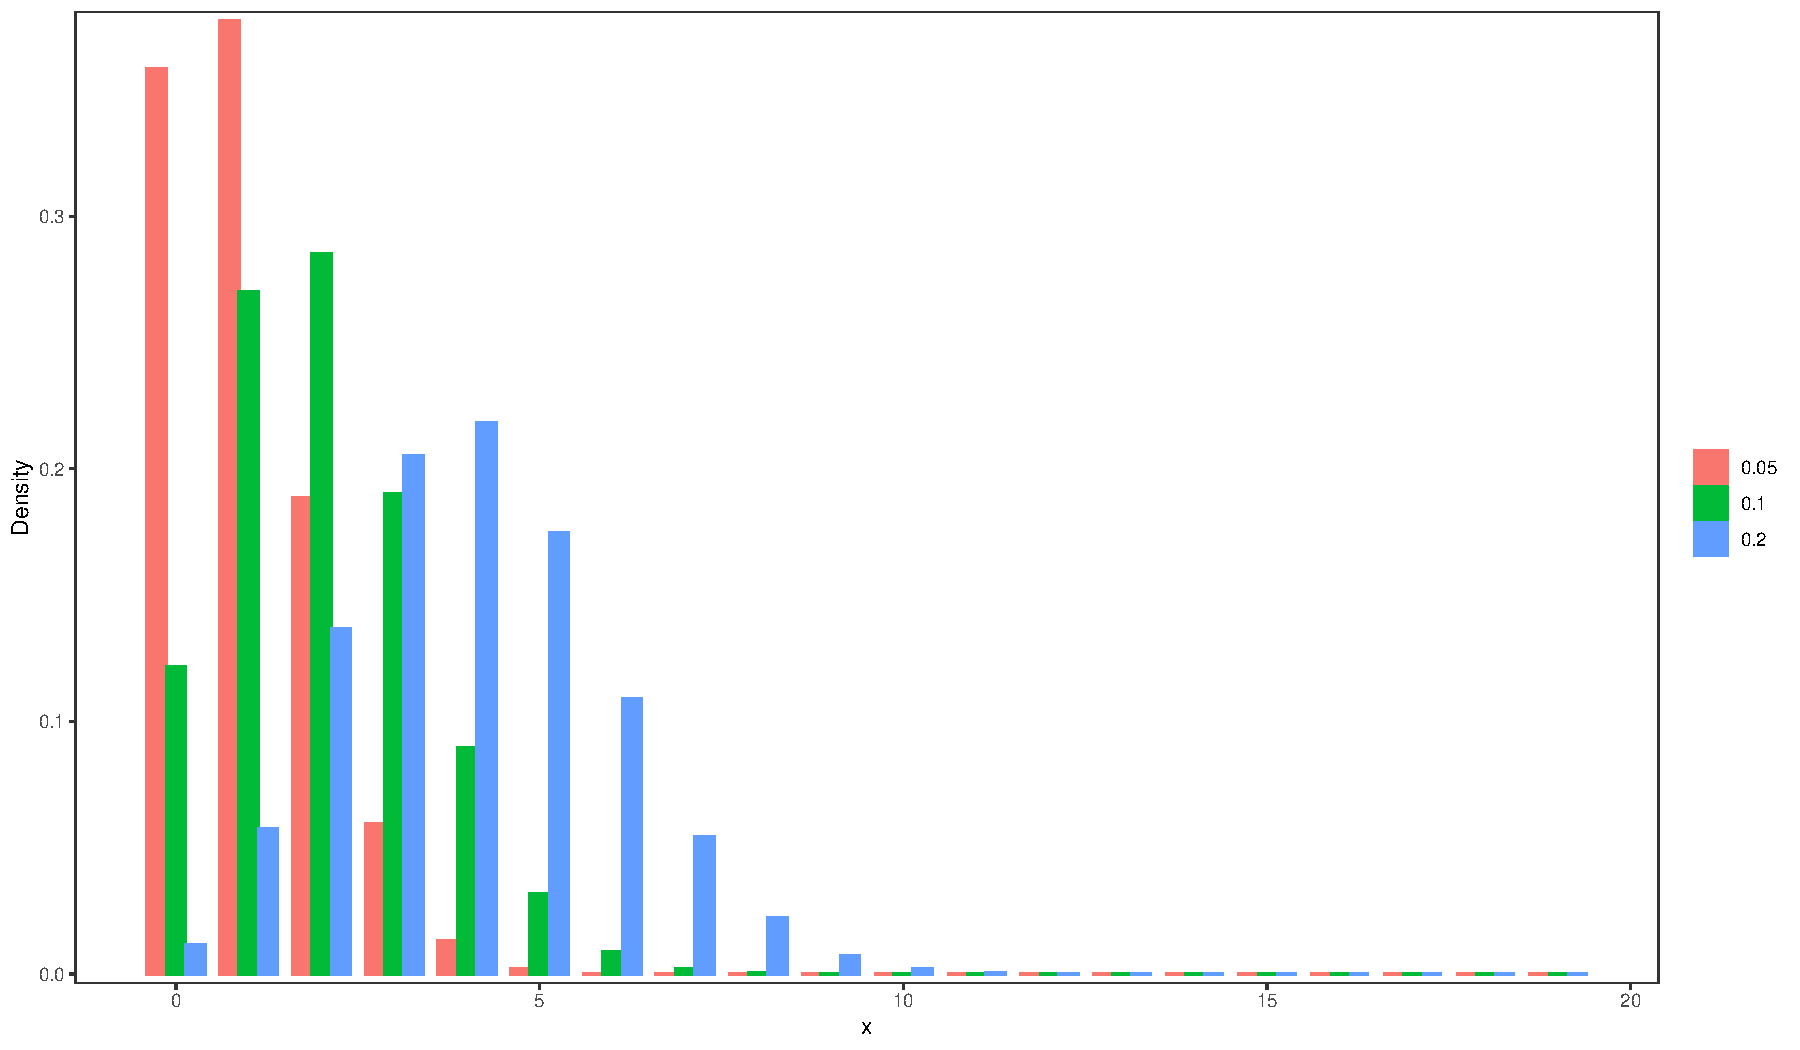
\includegraphics[scale=0.25]{figures/fig_1}
  \\
  \tiny 
\end{figure}

\tiny
 \begin{align}
 Pr(X=x)= \binom{n}{x}\theta^x(1-\theta)^{n-x} \\
 Pr(X=0)= \binom{20}{0}0.05^0(1-0.05)^{20-0} \approx 0.36
 \end{align}

\end{frame}

%----------------------------------------------------------------------%
\begin{frame}[fragile]
\frametitle{A Simple Covid Example}
\framesubtitle{Prior distribution}

\begin{itemize}
\item Other studies from various parts of the country indicate that the infection rate in comparable cities ranges from about 0.05 to 0.20, with an average prevalence of 0.10.
\item We will therefore use a prior distribution $p(\theta)$ 
\end{itemize}


\begin{align}
\theta \sim Beta(a,b)
\end{align}
where the density of a Beta takes the form of

\begin{align}
p(\theta)=\frac{\Gamma\left(a+b\right)}{\Gamma\left(a\right)\Gamma\left(b\right)}\theta^{a-1}\left(1-\theta\right)^{b-1}
\end{align}
with $a=2$ and $b=20$. Note that 

\begin{align}
E(\theta) =\frac{a}{a+b} =0.09 \\
Pr(0.05 < \theta < 0.20) = 0.66
\end{align}

\end{frame}
%----------------------------------------------------------------------%
\begin{frame}[fragile]
\frametitle{A Simple Covid Example}
\framesubtitle{Posterior distribution}

\begin{align}
\pi(\theta|X) &= \frac{f(X|\theta)p(\theta)}{m(X)} 
\end{align}


\begin{align}
\pi(\theta|X) &=  \binom{n}{x}\theta^x(1-\theta)^{n-x} \times\frac{\Gamma(a+b)}{\Gamma(a)\Gamma(b)}\theta^{a-1}(1-\theta)^{b-1}  \frac{1}{m(x)}
\end{align}

The marginal

\begin{align}
m(x) &= \int f(X|\theta)p(\theta)d\theta \\
 &= \int_0^1 \binom{n}{x}\theta^x(1-\theta)^{n-x} \times\frac{\Gamma(a+b)}{\Gamma(a)\Gamma(b)}\theta^{a-1}(1-\theta)^{b-1}  d\theta \\
 &= \binom{n}{x} \frac{\Gamma(a+b)}{\Gamma(a)\Gamma(b)} \int_0^1 \theta^{x+a-1}(1-\theta)^{n-x+b-1}  d\theta 
\end{align}

\end{frame}
%----------------------------------------------------------------------%
\begin{frame}[fragile]
\frametitle{A Simple Covid Example}
\framesubtitle{Posterior distribution}
The marginal (cont)
\begin{align}
%m(x) &= \int f(X|\theta)p(\theta)d\theta \\
 %&= \int_0^1 \binom{n}{x}\theta^x(1-\theta)^{n-x} \times\frac{\Gamma(a+b)}{\Gamma(a)\Gamma(b)}\theta^{a-1}(1-\theta)^{b-1}  d\theta \\
 %&= \binom{n}{x} \frac{\Gamma(a+b)}{\Gamma(a)\Gamma(b)} \int_0^1 \theta^{x+a-1}(1-\theta)^{n-x+b-1}  d\theta \\
 m(x) &= \binom{n}{x} \frac{\Gamma(a+b)}{\Gamma(a)\Gamma(b)}  \frac{\Gamma(a+x)\Gamma(b+n-x)}{\Gamma(a+b+n)} \int_0^1  \frac{\Gamma(a+b+n)}{\Gamma(a+x)\Gamma(b+n-x)} \theta^{x+a-1}(1-\theta)^{n-x+b-1}  d\theta \\
 &= \binom{n}{x} \frac{\Gamma(a+b)}{\Gamma(a)\Gamma(b)}  \frac{\Gamma(a+x)\Gamma(b+n-x)}{\Gamma(a+b+n)}
\end{align}

The posterior
\begin{align}
\pi(\theta|X) &=  \frac{\Gamma(a+b+n)}{\Gamma(a+x)\Gamma(b+n-x)} \theta^{x+a-1}(1-\theta)^{n-x+b-1}  \\
              &\sim Beta(a+x,b+n-x)
\end{align}

\end{frame}
%----------------------------------------------------------------------%
\begin{frame}[fragile]
\frametitle{A Simple Covid Example}
With the posterior we can calculate then any moment of the posterior distribution. For example suppose that for our study none of the sample of individuals is infected (x=0). Then the posterior is 

\begin{align}
\pi(\theta|X=0) &\sim Beta(2,40)
\end{align}

$a= 2$, $b=20$, $n=20$. Then

\begin{align}
\tiny
E(\theta|X=0)  &= \frac{a+x}{a+b+n} \\
               &= \frac{n}{a+b+n} \frac{x}{n} + \frac{a+b}{a+b+n} \frac{a}{a+b}  \\
               &= \frac{n}{a+b+n} \bar x + \frac{a+b}{a+b+n} \theta_{prior}  \\
               &= \frac{n}{a+b+n} 0 + \frac{a+b}{a+b+n} \frac{2}{22}  \\
 &= 0.048 
\end{align}

\end{frame}
%----------------------------------------------------------------------%
\begin{frame}[fragile]
\frametitle{A Simple Covid Example}

Since we have the full distribution we could calculate for example:
\begin{align}
mode(\theta|X) = 0.025 \\
Pr(\theta<0.10|X=0) &= 0.93
\end{align}

\begin{figure}[H] \centering
  \centering
  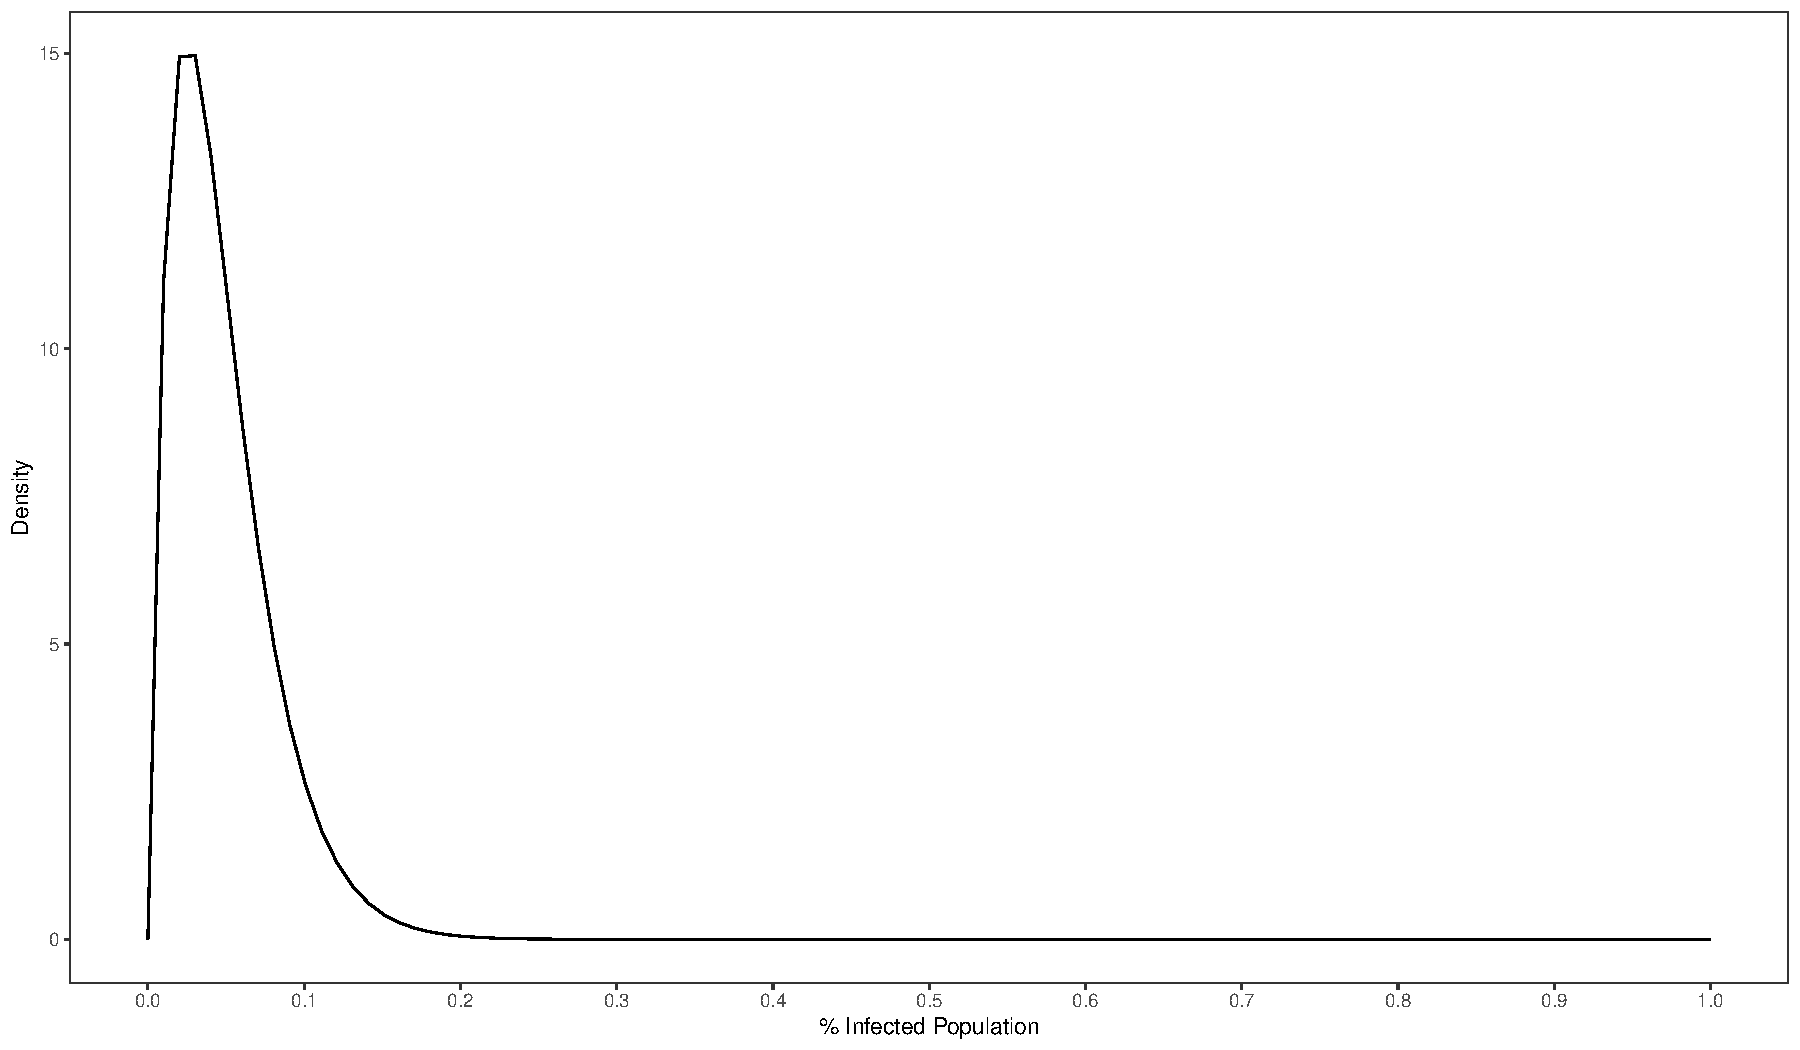
\includegraphics[scale=0.25]{figures/fig_2}
  \\
  \tiny 
\end{figure}


\end{frame}

%----------------------------------------------------------------------%
\begin{frame}
\frametitle{Bayes Theorem}
{\bf Conjugate Priors. Basic idea:}

\bigskip
\begin{itemize}
  \item $X\sim D(\theta)$ and $\theta \sim P(\lambda)$ $\rightarrow$ $\theta|X \sim P(\lambda')$
  \bigskip
  \item  $X\sim Bernoulli(\theta)$ and $\theta \sim Beta(a,b)$ $\rightarrow$ $\theta|X \sim Beta(a',b')$
  \bigskip
  \item  $X\sim N(\mu,\sigma)$ and $\theta \sim N(\mu_0,\sigma_0)$ $\rightarrow$ $\theta|X \sim N(\mu',\sigma')$
\end{itemize}

\end{frame}


%----------------------------------------------------------------------%
\section{Empirical Bayes}
%----------------------------------------------------------------------%
\subsection{Batting Averages}
%----------------------------------------------------------------------%
\begin{frame}[fragile]
\frametitle{Batting Averages}


We can model

\begin{align}
\text{Batting Average} \sim Binomial(n,\theta)
\end{align}

\begin{itemize}
\item where $n$ is the times at bat and $\theta$ is the proportion of successes
\item  We  use a conjugate prior for simplicity
\end{itemize}


\begin{align}
p(\theta) \sim Beta(\alpha_0,\beta_0)
\end{align}

The posterior is:
\begin{align}
\pi(\theta)\sim Beta(\alpha_0+hits,\beta_0+N-hits)
\end{align}

\end{frame}
%----------------------------------------------------------------------%
\begin{frame}[fragile]
\frametitle{Batting Averages}

Using last class data:

\bigskip
\begin{small}
\begin{verbatim}
## # A tibble: 6 x 4
##   name               H    AB average
##   <chr>          <int> <int>   <dbl>
## 1 Hank Aaron      3771 12364  0.305 
## 2 Tommie Aaron     216   944  0.229 
## 3 Andy Abad          2    21  0.0952
## 4 John Abadie       11    49  0.224 
## 5 Ed Abbaticchio   772  3044  0.254 
## 6 Fred Abbott      107   513  0.209
\end{verbatim}
\end{small}

\end{frame}

%----------------------------------------------------------------------%
\begin{frame}[fragile]
\frametitle{Batting Averages}

We are using batting averages to assess who are the best and worst batters
\begin{itemize}
  \item Best?
\end{itemize} 

\begin{small}
\begin{verbatim}
## # A tibble: 6 x 4
##   name             H    AB average
##   <chr>        <int> <int>   <dbl>
## 1 Roe Skidmore     1     1       1
## 2 Charlie Snow     1     1       1
## 3 Matt Tupman      1     1       1
## 4 Allie Watt       1     1       1
## 5 Al Wright        1     1       1
## 6 George Yantz     1     1       1
\end{verbatim}
\end{small}

\end{frame}

%----------------------------------------------------------------------%
\begin{frame}[fragile]
\frametitle{Batting Averages}

We are using batting averages to assess who are the best and worst batters

\begin{itemize}
  \item Worst?
\end{itemize}

\begin{small}
\begin{verbatim}
## # A tibble: 6 x 4
##   name                  H    AB average
##   <chr>             <int> <int>   <dbl>
## 1 Frank Abercrombie     0     4       0
## 2 Horace Allen          0     7       0
## 3 Pete Allen            0     4       0
## 4 Walter Alston         0     1       0
## 5 Bill Andrus           0     9       0
## 6 Wyman Andrus          0     4       0
\end{verbatim}
\end{small}

\end{frame}
%----------------------------------------------------------------------%
\begin{frame}[fragile]
\frametitle{Batting Averages}

Question: Can we use Bayesian stats to get a better estimate?


\begin{align}
X \sim Beta(\alpha_0,\beta_0)
\end{align}

\begin{itemize}
  \item We don't know $\alpha_0$ and $\beta_0$. We could use the fact that most batting averages are between .210 and .360. Select $\alpha_0$ and $\beta_0$ accordingly.
  \item Or we can use Empirical Bayes: estimate these parameters from the data
\end{itemize}


\end{frame}
%----------------------------------------------------------------------%
\begin{frame}[fragile]
\frametitle{Batting Averages}
Histogram of batting averages

\bigskip
\begin{figure}[H] \centering
  \centering
  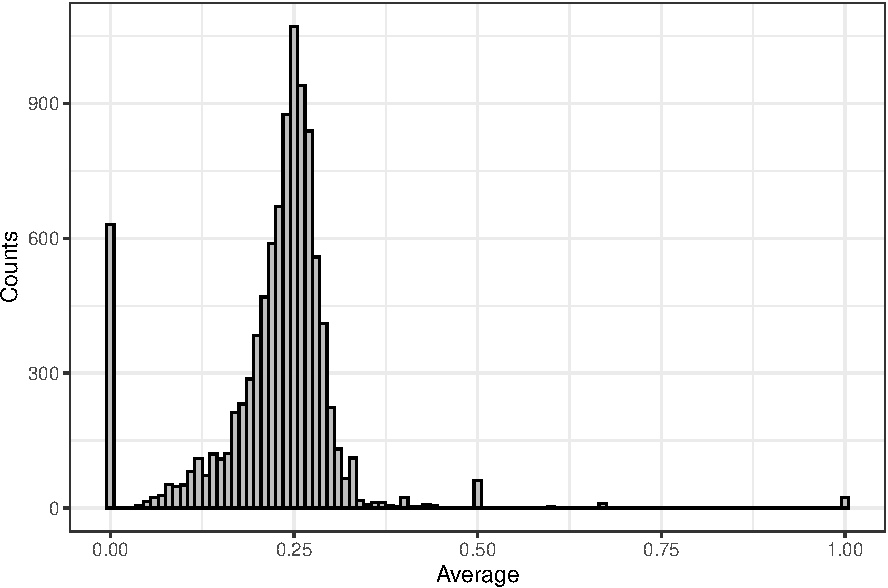
\includegraphics[scale=0.4]{figures/average_hist.pdf}
  \\
  \tiny 
\end{figure}



\end{frame}


%----------------------------------------------------------------------%
\begin{frame}[fragile]
\frametitle{Batting Averages}
Restrict our sample to those data points that are  informative (individuals that have gone at bat at least 500 times)

\bigskip

\begin{figure}[H] \centering
  \centering
  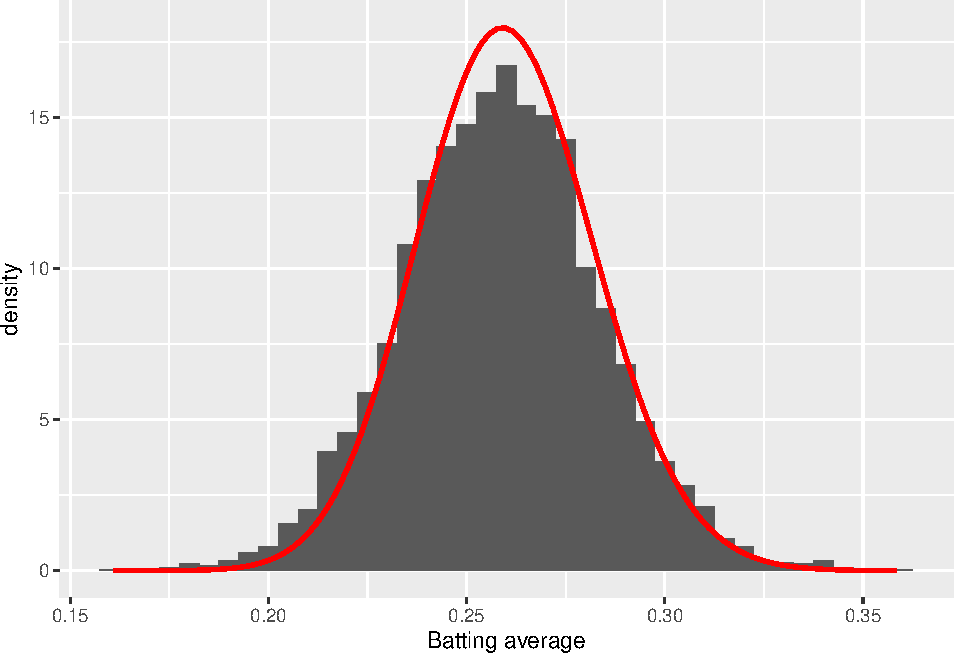
\includegraphics[scale=0.4]{figures/av_hist_w_mle.pdf}
  \\
  \tiny 
\end{figure}


\end{frame}

\begin{frame}[fragile]
\frametitle{Batting Averages}
How we find the parameters that find the red line $\rightarrow$ MLE! We know that

\begin{align}
f(x_i|\alpha_0,\beta_0)=\frac{\Gamma(\alpha_0+\beta_0)}{\Gamma(\alpha_0)\Gamma(\beta_0)}x_i^{\alpha_0-1}\left(1-x_i\right)^{\beta_0-1}
\end{align}

The log likelihood 
\begin{footnotesize}
\begin{align}
l(\alpha_0,\beta_0|X) = n . log(\frac{\Gamma(\alpha_0+\beta_0)}{\Gamma(\alpha_0)\Gamma(\beta_0)}) + \sum_{i=1}^n ((\alpha_0-1)log(x_i)+(\beta_0-1)log(1-x_i))
\end{align}
\end{footnotesize}


In \texttt{R}
\footnotesize
\begin{Shaded}
\begin{Highlighting}[]
\CommentTok{\# log{-}likelihood function}
\NormalTok{ll \textless{}{-}}\StringTok{ }\ControlFlowTok{function}\NormalTok{(alpha, beta) \{}
\OperatorTok{{-}}\KeywordTok{sum}\NormalTok{(VGAM}\OperatorTok{::}\KeywordTok{dbetabinom.ab}\NormalTok{(x, total, alpha, beta, }\DataTypeTok{log =} \OtherTok{TRUE}\NormalTok{))}
\NormalTok{\}}
\CommentTok{\# maximum likelihood estimation}
\NormalTok{m \textless{}{-}}\StringTok{ }\KeywordTok{mle}\NormalTok{(ll, }\DataTypeTok{start =} \KeywordTok{list}\NormalTok{(}\DataTypeTok{alpha =} \DecValTok{1}\NormalTok{, }\DataTypeTok{beta =} \DecValTok{10}\NormalTok{), }
\DataTypeTok{method =} \StringTok{"L{-}BFGS{-}B"}\NormalTok{, }\DataTypeTok{lower =} \KeywordTok{c}\NormalTok{(}\FloatTok{0.0001}\NormalTok{, }\FloatTok{.1}\NormalTok{))}
\NormalTok{ab \textless{}{-}}\StringTok{ }\KeywordTok{coef}\NormalTok{(m) }
\end{Highlighting}
\end{Shaded}


\end{frame}
%----------------------------------------------------------------------%
\begin{frame}[fragile]
\frametitle{Batting Averages}
\footnotesize
\begin{Shaded}
\begin{Highlighting}[]
\NormalTok{alpha0 \textless{}{-}}\StringTok{ }\NormalTok{ab[}\DecValTok{1}\NormalTok{]}
101.7319 
\NormalTok{beta0 \textless{}{-}}\StringTok{ }\NormalTok{ab[}\DecValTok{2}\NormalTok{]}
289.046 
\end{Highlighting}
\end{Shaded}



\begin{figure}[H] \centering
  \centering
  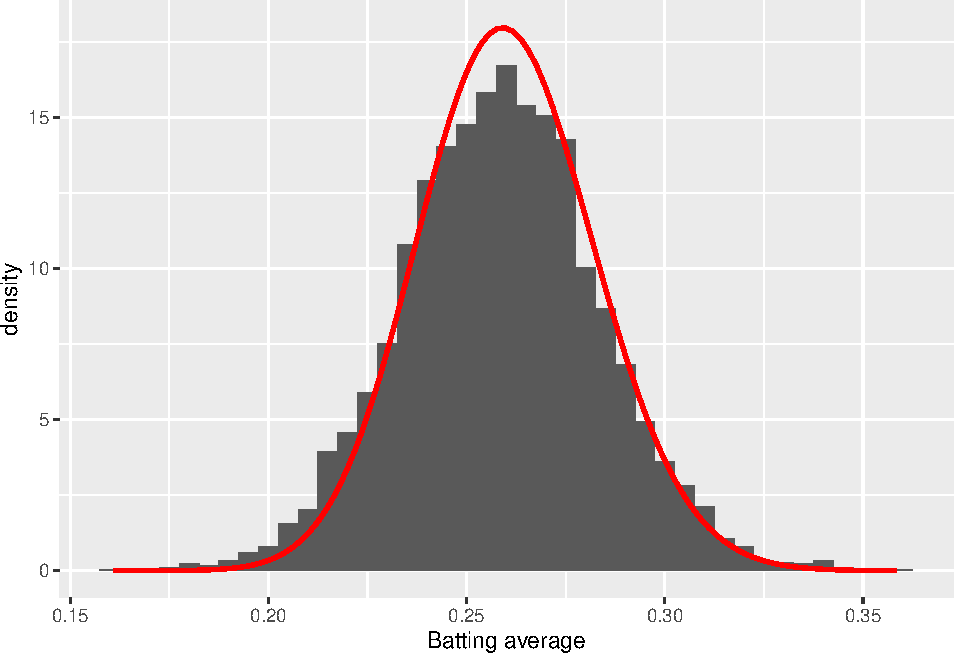
\includegraphics[scale=0.4]{figures/av_hist_w_mle.pdf}
  \\
  \tiny 
\end{figure}


\end{frame}
%----------------------------------------------------------------------%
\begin{frame}[fragile]
\frametitle{Batting Averages}

We can use the estimated average based on the posterior mean

\begin{align}
E(\theta|X)=\frac{\alpha+hits}{\alpha+\beta+N}
\end{align}


\begin{itemize}
  \item And ask again: who are the best batters by this improved estimate?
\end{itemize}


\begin{footnotesize}
\begin{verbatim}
## # A tibble: 5 x 5
##   name                     H    AB average eb_estimate
##   <chr>                <int> <int>   <dbl>       <dbl>
## 1 Rogers Hornsby        2930  8173   0.358       0.354
## 2 Shoeless Joe Jackson  1772  4981   0.356       0.349
## 3 Ed Delahanty          2597  7510   0.346       0.342
## 4 Billy Hamilton        2164  6283   0.344       0.339
## 5 Willie Keeler         2932  8591   0.341       0.338
\end{verbatim}
\end{footnotesize}

\end{frame}
%----------------------------------------------------------------------%
\begin{frame}[fragile]
\frametitle{Batting Averages}

We can use the estimated average based on the posterior mean

\begin{align}
E(\theta|X)=\frac{\alpha+hits}{\alpha+\beta+N}
\end{align}


\begin{itemize}
\item Who are the \emph{worst} batters?
\end{itemize}
\begin{footnotesize}
\begin{verbatim}
## # A tibble: 5 x 5
##   name                H    AB average eb_estimate
##   <chr>           <int> <int>   <dbl>       <dbl>
## 1 Bill Bergen       516  3028   0.170       0.181
## 2 Ray Oyler         221  1265   0.175       0.195
## 3 Henry Easterday   203  1129   0.180       0.201
## 4 John Vukovich      90   559   0.161       0.202
## 5 George Baker       74   474   0.156       0.203
\end{verbatim}
\end{footnotesize}

\end{frame}
%----------------------------------------------------------------------%
\begin{frame}[fragile]
\frametitle{Batting Averages}

We can see how EB changed all of the batting average estimates:

\begin{figure}[H] \centering
  \centering
  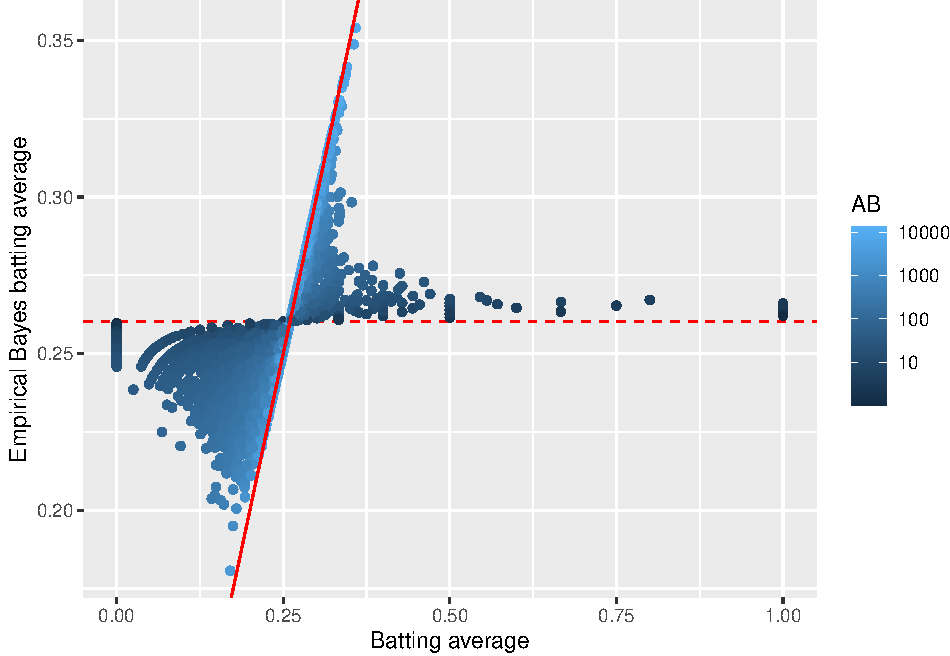
\includegraphics[scale=0.5]{figures/shrinkage_averages}
  \\
  \tiny 
\end{figure}



\end{frame}

%----------------------------------------------------------------------%
\subsection{Predicting Batting Averages}
%----------------------------------------------------------------------%
\begin{frame}[fragile]
\frametitle{Predicting Batting Averages}

\begin{itemize}
\item Now supposed you want to know the end of season final batting average of players, after observing them their 45 first times at bat.
\end{itemize}


\begin{table}[H]
\begin{tabular}{lcc}
\hline
\hline
Player & Observed & Final \\
\hline
1 & 0.395 & 0.346 \\
2 & 0.355 & 0.279 \\
3 & 0.313 & 0.276 \\
4 & 0.291 & 0.266 \\
5 & 0.247 & 0.271 \\
6 & 0.224 & 0.266 \\
7 & 0.175 & 0.318 \\
\hline
\hline
\end{tabular}
\end{table}
\end{frame}
%----------------------------------------------------------------------%
\begin{frame}[fragile]
\frametitle{Predicting Batting Averages}

\begin{itemize}
\item Recall that we can think each time at bat can be thought as a binomial trial, with $\theta$ the probability of success equal to the player's true batting average.
\item With 45 trials, we can ``reasonably'' use a Normal Approximation.
\end{itemize}

\begin{align}
  X_i \sim N(\theta_i,\sigma^2)
\end{align}
where

\begin{itemize}
  \item $\theta_i$ is the true batting average for player $i$
  \item $\sigma^2$ is the known variance that equals $(0.0659)^2$
\end{itemize}
We are going to use also a normal prior

\begin{align}
  \theta_i \sim N(\mu,\tau^2)
\end{align}

\end{frame}
%----------------------------------------------------------------------%
\begin{frame}[fragile]
\frametitle{Predicting Batting Averages}
With this model the posterior mean for $\theta_i$ is $E(\theta_i|X_i)$

\begin{align}
E(\theta_i|X_i)=\frac{\sigma^2}{\sigma^2+\tau^2}\mu + \frac{\tau^2}{\sigma^2+\tau^2} X_i
\end{align}
Note that the marginal of $X_i$

\begin{align}
m(X_i)\sim N(\mu,\sigma^2+\tau^2)\,\,\,i=1,\dots,n
\end{align}

with these we can construct estimates of $E(\theta_i|X_i)$, note that

\begin{align}
E(\bar X)&=\mu \\
E\left[ \frac{(n-3)\sigma^2}{\sum(X_i-\bar X)^2}\right]&=\frac{\sigma^2}{\sigma^2+\tau^2}
\end{align}



\end{frame}
%----------------------------------------------------------------------%
\begin{frame}[fragile]
\frametitle{Predicting Batting Averages}

The empirical Bayes estimator of $\theta_i$ is then
\begin{footnotesize}
  \begin{align}
    \delta(X_i)= \left[ \frac{(n-3)\sigma^2}{\sum((X_i-\bar X)^2}\right] \bar X + \left[ 1- \frac{(n-3)\sigma^2}{\sum((X_i-\bar X)^2}\right] X_i
  \end{align}
\end{footnotesize}


\begin{table}[]
\begin{tabular}{lcccc}
\hline
\hline
Player & Observed & Final & Empirical Bayes  \\
\hline
1      & 0.395    & 0.346 & 0.341            \\
2      & 0.355    & 0.279 & 0.321            \\
3      & 0.313    & 0.276 & 0.299            \\
4      & 0.291    & 0.266 & 0.288            \\
5      & 0.247    & 0.271 & 0.266            \\
6      & 0.224    & 0.266 & 0.255            \\
7      & 0.175    & 0.318 & 0.230           \\
\hline
\hline
\end{tabular}
\end{table}

\begin{itemize}
\item RMSE Observed 6.861903
\item RMSE EB 3.918203
\end{itemize}
\end{frame}
%----------------------------------------------------------------------%
\begin{frame}[fragile]
\frametitle{Predicting Batting Averages}

\begin{figure}[H] \centering
  \centering
  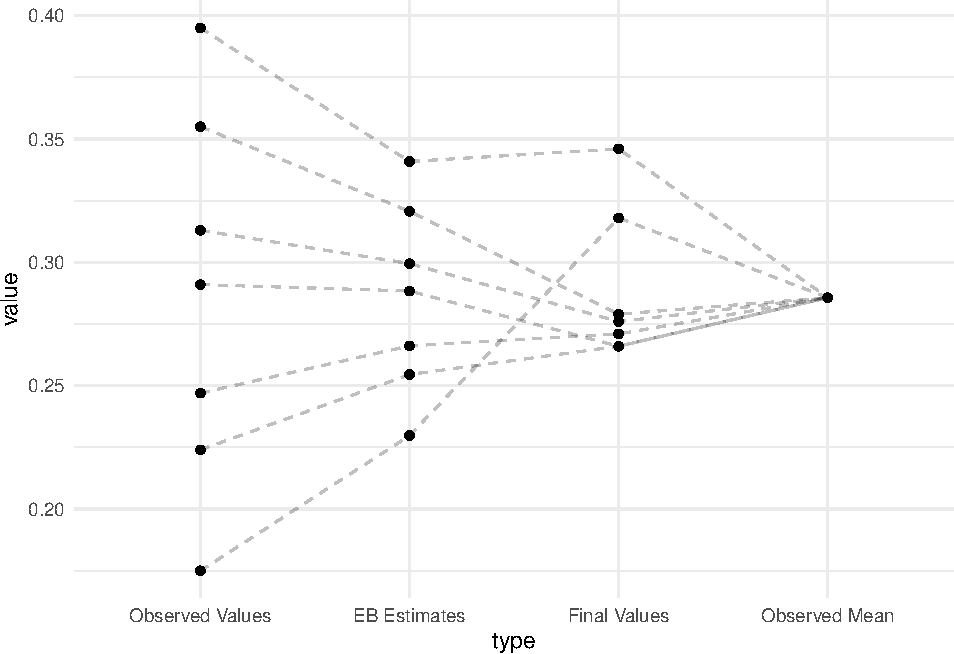
\includegraphics[scale=0.5]{figures/shrinkage_future}
  \\
  \tiny 
\end{figure}



\end{frame}



%----------------------------------------------------------------------%
%----------------------------------------------------------------------%
\begin{frame}
\frametitle{Review \& Next Steps}
  
  \begin{itemize} 
    \item Recap Bayesian
    \medskip
    \item Empirical Bayes Examples
    
  \bigskip  

\item  Next couple of classes we are going to focus on 
  \begin{itemize}
      \item Concepts underlying spatial data: points, lines, polygons, reference systems
      \medskip
      \item Plotting and describing spatial data
      \medskip
      \item Econometric models for spatial data
\end{itemize}

\bigskip  
\item Questions? Questions about software? 

\end{itemize}
\end{frame}

%----------------------------------------------------------------------%

%----------------------------------------------------------------------%

\section{Further Readings}
%----------------------------------------------------------------------%
\begin{frame}
\frametitle{Further Readings}
\footnotesize
\begin{itemize}
  \item Casella, G., \& Berger, R. L. (2002). Statistical inference (Vol. 2, pp. 337-472). Pacific Grove, CA: Duxbury. Chapter 7
  \medskip
  \item Casella, G. (1985). An introduction to empirical Bayes data analysis. The American Statistician, 39(2), 83-87.
  \medskip
  \item Robinson, D. (2017). Introduction to Empirical Bayes: Examples from Baseball Statistics. 2017.
  \end{itemize}

\end{frame}



%----------------------------------------------------------------------%
%----------------------------------------------------------------------%
\end{document}
%----------------------------------------------------------------------%
%----------------------------------------------------------------------%

